%%%%%%%%%%%%%%%%%%%%%%
\begin{frame}{Introduction}
The algorithm was named \emph{ComTector} because it is a Community Detector algorithm. 
\vskip 0.3cm
The algorithm was designed by:

\vskip 0.3cm

\begin{itemize}
  \item Nan Du -  \href{mailto:dunan@bupt.edu.cn}{dunan@bupt.edu.cn}
  \item Bin Wu -  \href{mailto:wubin@bupt.edu.cn}{wubin@bupt.edu.cn}
  \item Xin Pei -  \href{mailto:peixin@tseg.org}{peixin@tseg.org}
  \item Bai Wang -  \href{mailto:wangbai@bupt.edu.cn}{wangbai@bupt.edu.cn}
  \item Liutong Xu -  \href{mailto:xliutong@bupt.edu.cn}{xliutong@bupt.edu.cn}
  
\end{itemize}


\end{frame}

%%%%%%%%%%%%%%%%%%%%%%
\begin{frame}{Introduction}
The algorithm which will be presented is more efficient and accurate than the other known algorithm in community detection because:

\vskip 0.5cm

\begin{itemize}
  \item It is focused on \emph{Large-Scale Social Networks}
  \item It takes advantages of the \emph{sparsity} of the Social Adjacent Matrixes
  \item It considers the \emph{overlapping} nature of the social relationships
\end{itemize}

\vskip 1cm

There is no need of a-priori knowledge of the network communities.

\end{frame}

%%%%%%%%%%%%%%%%%%%%
\begin{frame}{Presentation structure}
\vskip 0.5cm
This is the structure of the paper and the presentation will follow it.
\vskip 0.5cm

\begin{center}
	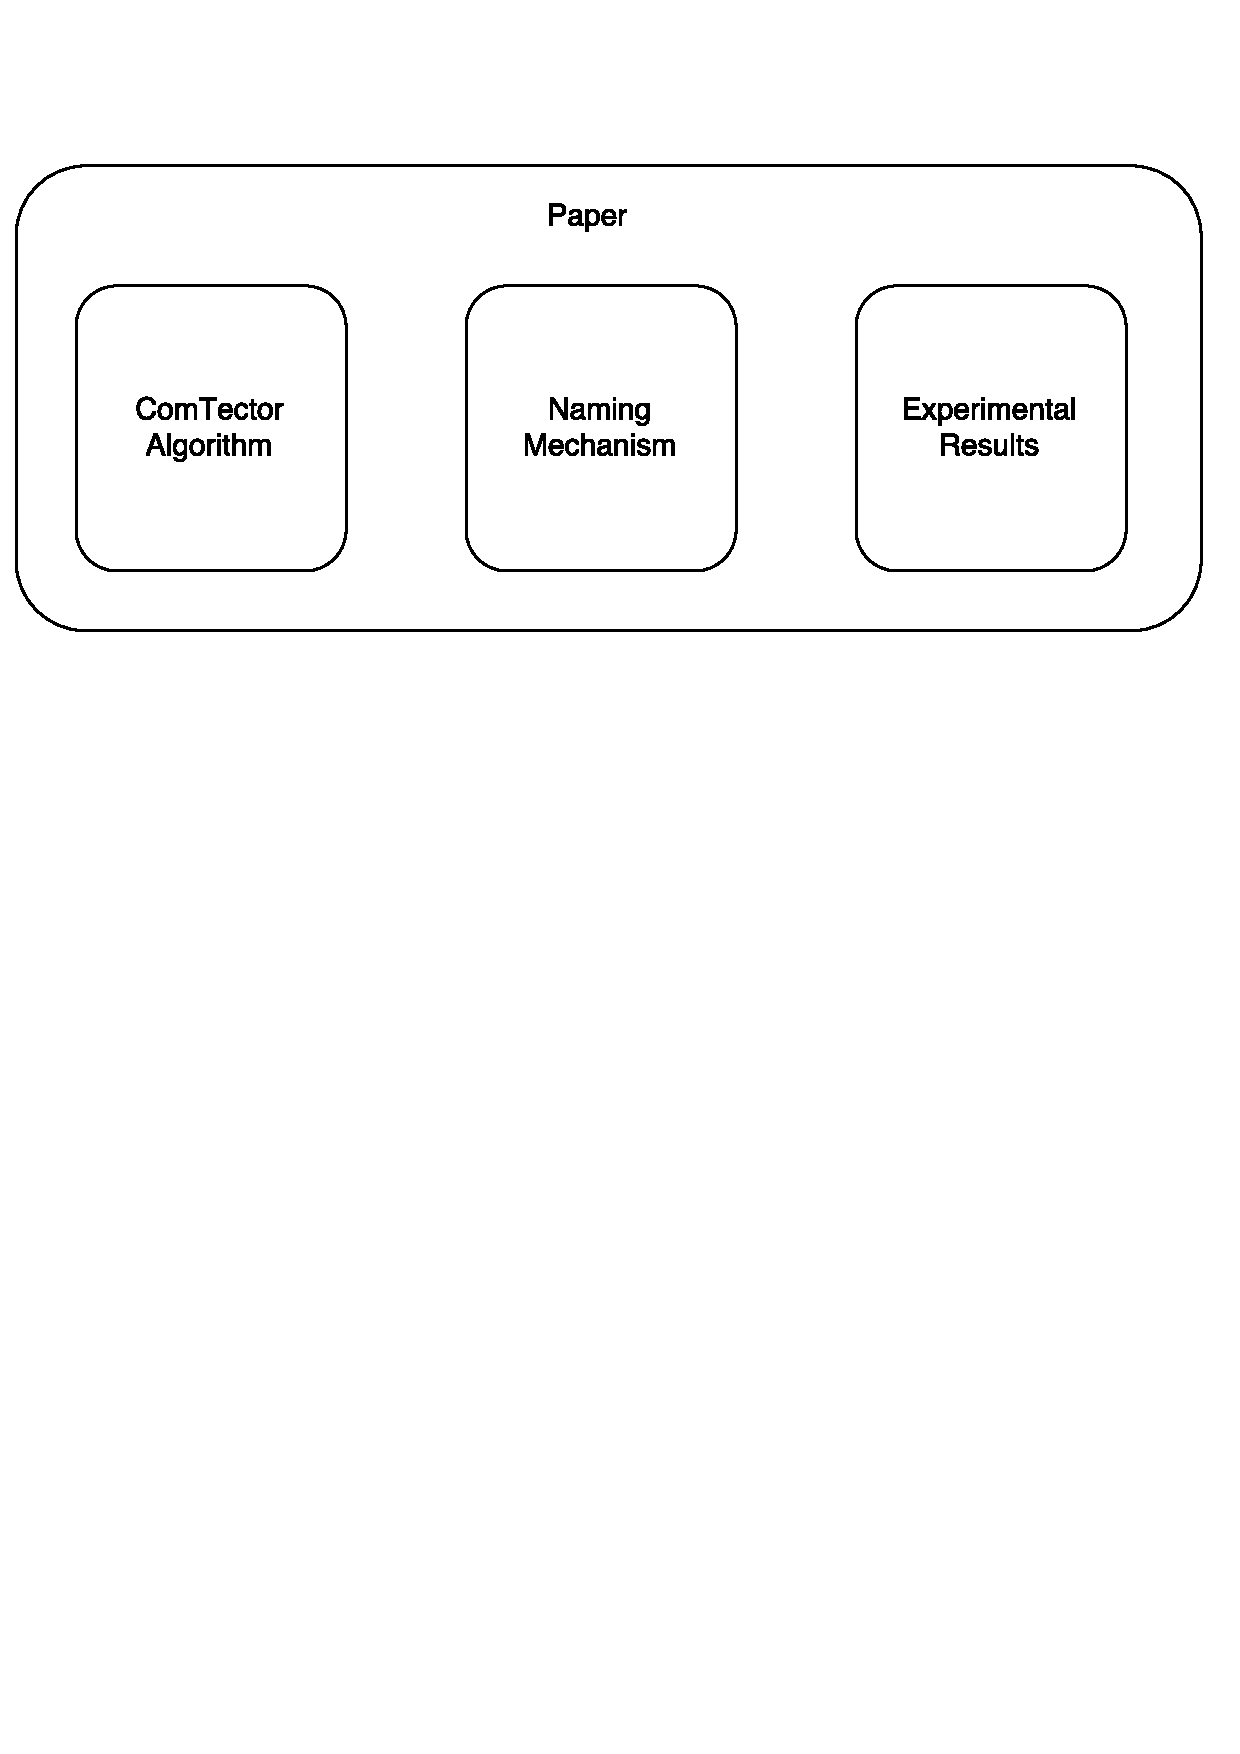
\includegraphics[height=3.5cm]{images/paperStructure.pdf}
\end{center}

In the paper the ComTector presentation is structured using the bottom-up approach, while in this presentation it is top-down, in order to make an initially clearer global vision of the algorithm.

\end{frame}